\documentclass[times, utf8, zavrsni, numeric]{fer}
\usepackage{booktabs}
\usepackage{listingsutf8}
\usepackage[titletoc,page]{appendix}
\captionsetup[lstlisting]{position=bottom}
\addto\captionsenglish{%
  \renewcommand{\figurename}{Slika}%
  \renewcommand{\contentsname}{Sadržaj}
  \renewcommand{\appendixname}{Dodatak}
  \renewcommand\tablename{Tablica}
  \renewcommand\bibname{Literatura}
  \renewcommand{\lstlistingname}{Primjer}
}
\usepackage{listings}
\usepackage{color}

\definecolor{dkgreen}{rgb}{0,0.6,0}
\definecolor{gray}{rgb}{0.5,0.5,0.5}
\definecolor{mauve}{rgb}{0.58,0,0.82}

\lstset{frame=tb,
  language=Java,
  aboveskip=3mm,
  belowskip=3mm,
  showstringspaces=false,
  columns=flexible,
  captionpos=b,
  basicstyle={\small\ttfamily},
  numbers=none,
  numberstyle=\tiny\color{gray},
  keywordstyle=\color{blue},
  commentstyle=\color{dkgreen},
  stringstyle=\color{mauve},
  breaklines=true,
  breakatwhitespace=true,
  tabsize=3
}
%\lstset{language=Java,
% basicstyle=\tiny\tt,
% showspaces=false,
% showstringspaces=false,
% breaklines=true
% }
\lstset{
    literate=%
    {ć}{{\'c}}1
    {č}{{\v{c}}}1
    {đ}{{\dj{}}}1
    {š}{{\v{s}}}1
    {ž}{{\v{z}}}1
    {Ć}{{\'C}}1
    {Č}{{\v{C}}}1
    {Đ}{{\DJ{}}}1
    {Š}{{\v{S}}}1
    {Ž}{{\v{Z}}}1
}
\begin{document}

% TODO: Navedite broj rada.
\thesisnumber{1337}

% TODO: Navedite naslov rada.
\title{Obrada podataka tehnologijom Apache Spark}

% TODO: Navedite vaše ime i prezime.
\author{Martin Matak}

\maketitle

% Ispis stranice s napomenom o umetanju izvornika rada. Uklonite naredbu \izvornik ako želite izbaciti tu stranicu.
\izvornik{Na ovoj stranici se nalazi izvornik.}

% Dodavanje zahvale ili prazne stranice. Ako ne želite dodati zahvalu, naredbu ostavite radi prazne stranice.
\zahvala{Zahvala - TODO \ldots :)}

\tableofcontents

\chapter{Uvod}
\section{Motivacija}
%Literatura: http://mob.hr/samsung-galaxy-s4-skrivene-mogucnosti-senzori-i-octa-5-benchmark/
Skoro pa svaka osoba danas posjeduje mobilni uređaj, a neke osobe posjeduju i više njih. Pametni mobilni uređaji postaju neizostavan dodatak svakog modernog čovjeka. Prošlo je vrijeme kada su mobilni uređaji jedino služili za pozive i SMS poruke. Današnji mobilni uređaji imaju puno više mogućnosti. Osim što je zadržana funkcionalnost uspostavljanja poziva i slanja poruka, postoji mogućnost povezivanja na internet, orijentaciju u prostoru, mjerenje brzine itd. Da bi sve te stvari bile moguće, većina današnjih mobilnih uređaja u sebi sadrži senzore koji su navedeni i opisani u tablici \ref{tbl:senzori}.

\begin{table}[htb]
\caption{Neki od senzora u današnjim mobilnim uređajima.}
\label{tbl:senzori}
\centering
\begin{tabular}{l p{8cm}}
\hline
Senzor & Opis \\
\hline
Akcelerometar & Elektromehanička komponenta koja mjeri sile ubrzanja. \\
Barometar & Mehanički senzor za mjerenje atmosferskog pritiska (na trenutnoj lokaciji uređaja).\\
Senzor svjetlosti & Mjeri intenzitet, tj. jačinu svjetlosti i uglavnom se nalazi s prednje strane uređaja, iznad ekrana. \\
Senzor blizine & U stanju prepoznati situacije kada mu neki objekt stoji u blizini - ovo omogućava automatske pozive prilikom primicanja telefona licu uz zaključavanje telefona da bi onemogućili slučajno prekidanje poziva uhom ili slično.\\
Senzor gestikulacije & Prepoznaje kretnje ruke tako što detektira infracrvene zrake koje se reflektiraju, odnosno omogućuje djelomično upravljanje telefonom bez doticanja ekrana.\\
Žiroskop & Uređaj koji se koristi za navigaciju i mjerenje kutne brzine.\\
Geomagnetski senzor & Mjeri okolno geomagnetsko polje za sve tri fizičke osi, odnosno služi kao kompas na mobilnim uređajima. \\
\emph{Hall Sensor} & Magnetski senzor zadužen za prepoznavanje je li  maska telefona zatvorena ili otvorena. \\
\hline
\end{tabular}
\end{table}

Pretpostavimo da je mobilni uređaj spojen na internet i da svakih nekoliko sekundi pošalje vrijednost koju u tom trenutku mjeri pojedini senzor. U samo jednom danu može se skupiti dosta podataka. A što kada to ne bi radili za jedan uređaj nego za sve izdane uređaje nekog modela? Količina podataka bi jako brzo narasla.

Kako količina podataka postaje sve veća, dolazimo do pojma \emph{Velika količina podataka} \engl{Big Data}. U današnje vrijeme postoji više podataka u digitalnom obliku nego što ih je ikada bilo. Jedan od zanimljivijih izazova je kako ih djelotvorno obraditi i zaključiti nešto iz toga, odnosno kako od te velike količine podataka doći do nekih pametnih zaključaka i nešto novo naučiti.

Tehnologija \emph{Apache Spark} je tehnologija otvorenog koda \engl{open source} koja omogućava pisanje programa za obradu podataka u tri programskih jezika: Java, Python i Scala. Dodatno, postoji i mogućnost interaktivnog rada. \\
U okviru ovog rada proučeni su neki djelovi ove tehnologije, razrađeno nekoliko konkretnih primjera obrade podataka te ostvarena programska rješenja koja obavljaju tu obradu koristeći tehnologiju \emph{Apache Spark}.

Svi primjeri su napisani u programskom jeziku Java.

\section{Osnovni gradivni elementi}
Tehnologija \emph{Apache Spark} je pisana u programskom jeziku Scala i izvršava se na \emph{Javinom virtualnom stroju} (engl. \emph{Java Virtual Machine}, kratica JVM). Instalacija na osobno računalo je objašnjena u dodatku \ref{ch:instalacijaSpark}. Opisi nekih direktorija i datoteka koje se dobiju instalacijom dani su u tablici \ref{tbl:installPackage}. Zanimljivo je spomenuti da postoji interaktivna ljuska \emph{Spark shell}, ali isključivo za programske jezike Python i Scala. Datoteke u direktoriju \emph{bin} služe upravo za to. Budući da je ovaj rad ograničen isključivo na programski jezik Java, a u ovom trenutku takva interaktivna ljuska još ne postoji, interaktivna ljuska nije detaljnije obrađena. Više informacija potražiti u \cite{learningSpark}.

\begin{table}[htb]
\caption{Dio datoteka i direktorija dobivenih instalacijom.}
\label{tbl:installPackage}
\centering
\begin{tabular}{l p{8cm}}
\hline
Datoteka ili direktorij & Opis \\
\hline
\emph{bin} & Sadrži izvršive datoteke koje se koriste za interaktivni rad s tehnologijom \emph{Apache Spark}.\\
\emph{core, streaming, python, ...} & Sadrži glavne komponente tehnologije. \\
\emph{README.md} & Sadrži kratke instrukcije za upoznavanje s tehnologijom.\\
\emph{examples} & Sastoji se od nekoliko jednostavnih primjera koje pomažu korisniku da se uhoda i što bezbolnije nauči koristiti programsko sučelje koje tehnologija pruža. \\
\hline
\end{tabular}
\end{table}

Osnovna programska apstrakcija s kojom tehnologija \emph{Apache Spark} radi je \emph{otporni raspodijeljeni skup podataka} (engl. \emph{resilient distributed dataset}, kratica RDD) \cite{workingSets}.
Atribut \emph{otproni} znači da se može ponovno rekonstruirati u slučaju da se particija uništi. \emph{Raspodijeljeni} znači da je to skup podataka koji se nalazi na računalima (jednom ili više njih) i moguće ga je paralelno obrađivati. \emph{Skup podataka} znači da predstavlja nekakvu kolekciju podataka. Tehnologija \emph{Apache Spark} nudi bogato programsko sučelje za rad s tim skupovima podataka.

\begin{figure}[htb]
\centering
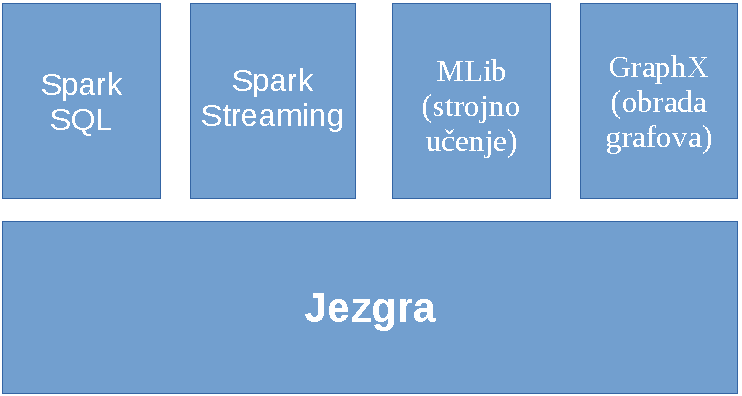
\includegraphics[width=10cm]{img/gradivniElementiCropped.pdf}
\caption{Osnovni elementi tehnologije \emph{Apache Spark}.}
\label{fig:spark-stack}
\end{figure}
\pagebreak
Tehnologija se sastoji od nekoliko ključnih elemenata koji su u tablici \ref{tbl:gradivniElementi} samo nabrojani i opisani rečenicom ili dvije. Detaljnije objašnjenje nalazi se u kasnijim poglavljima. Slika \ref{fig:spark-stack} predstavlja osnovne elemente tehnologije \emph{Apache Spark}.

\begin{table}[htb]
\caption{Dio datoteka i direktorija dobivenih instalacijom.}
\label{tbl:gradivniElementi}
\centering
\begin{tabular}{l p{8cm}}
\hline
Komponenta & Opis \\
\hline
\emph{Spark SQL} & Omogućuje rad s bilo kakvim strukturiranim podatcima, primjerice \emph{JSON}. Također, nudi i mogućnost izvršavanja \emph{SQL} naredbi. \\
\emph{Spark Streaming} & Komponenta zadužena za rad s tokovima podataka. \\
\emph{MLib} & Koristi se za postupke strojnog učenja. \\
\emph{GraphX} & Biblioteka za obradu grafova (npr. graf prijatelja na društvenoj mreži).\\
\hline
\end{tabular}
\end{table}

\chapter{Prvi programi}
U ovom poglavlju opisano je kako napisati osnovni program koristeći tehnologiju \emph{Apache Spark}. Također je opisano i od čega se takav program sastoji i koja je uloga pojedine komponente programa. Primjer koji se obrađuje je primjer \ref{lst:brojanjeRijeci}, a svodi se na jednostavan algoritam brojanja riječi.

\section{Postavljanje temelja}
\subsection{Osnovni elementi aplikacije}
Općenito govoreći, svaka se Spark aplikacija sastoji  od nekoliko komponenata. Prva komponenta koju ćemo spomenuti je program koji se izvršava - onaj čija je \texttt{main} metoda pokrenuta, odnosno onaj koji pokreće obradu podataka. Taj program naziva se pozivajući program \engl{driver}. Pozivajući program s podatcima priča kroz "tunel" koji se naziva \emph{SparkContext}.

\begin{figure}[htb]
\centering
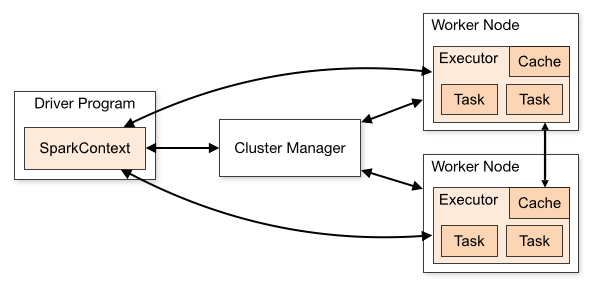
\includegraphics[width=10cm]{img/cluster-overview.png}
\caption{Prikaz elemenata aplikacije. Preuzeto s \protect\url{http://spark.apache.org/docs/latest/cluster-overview.html}.}
\label{fig:cluster-overview}
\end{figure}

Budući da je tehnologija \emph{Apache Spark} namijenjena za paralelnu obradu podataka, postoje još dvije komponente koje pridonose upravo tome. Pojedino računalo u \emph{grozdu} \engl{cluster} naziva se \emph{radnim čvorom} \engl{worker node}, a proces koji se izvršava na pojedinom računalu naziva se \emph{radnik} \engl{executor}. Dozvoljeno je da \emph{radnici} međusobno komuniciraju. U cijeloj priči može, a i ne mora eksplicitno biti uključen \emph{upravitelj grozdom} \engl{cluster manager}.
Opisana struktura prikazana je na slici \ref{fig:cluster-overview}.

\subsection{Korištenje tehnologije Apache Spark kroz programski jezik Java}
Kako bi mogli pisati Spark programe u programskom jeziku Java, potrebno je povezati svoju aplikaciju s \texttt{spark-core} artefaktom s Mavena. Za postavljanje i instalaciju Mavena konzultirati \url{https://maven.apache.org/install.html} i knjigu \cite{marcupic}. Za vrijeme pisanja ovog rada, najnovija verzija Sparka je 1.6.1, a odgovarajuće Maven koordinate su:
\begin{lstlisting}[language=bash, basicstyle=\small]
groupId = org.apache.spark
artifactId = spark-core_2.10
version = 1.6.1
\end{lstlisting}

Odgovarajuća \texttt{pom.xml} datoteka nalazi se u dodatku \ref{ch:datotekapomXML}.
Jednom kada je \texttt{pom.xml} datoteka namještena i projekt uspješno povezan sa \texttt{spark-core}, sve što je još potrebno jest inicijalizirati \emph{SparkContext} i napisati prvu aplikaciju. U primjeru \ref{lst:brojanjeRijeci} nalazi se jednostavna aplikacija koja jedino što radi je broji koliko puta se pojedina riječ pojavljuje u tekstualnoj datoteci.
\begin{lstlisting}[numbers=left, label={lst:brojanjeRijeci}, caption={Program koji broji koliko se puta koja riječ pojavljuje u datoteci.}]
package hr.fer.zemris;

import java.util.Arrays;

import org.apache.spark.SparkConf;
import org.apache.spark.api.java.*;
import org.apache.spark.api.java.function.*;

import scala.Tuple2;

/**
 * Razred ima svrhu prikazati osnovnu funkcionalnost Spark
 * tehnologije na primjeru prebrojavanja riječi
 * u tekstualnoj datoteci. Kao rezultat program će
 * zapisati u tekstualnu datoteku koja riječ se koliko puta
 * ponavlja. Očekuje se dva argumenta kroz naredbeni 
 * redak, a to su putanja do tekstualne datoteke u kojoj
 * treba izbrojati riječi i putanja do direktorija
 * u koji će se zapisati rezultat.
 *
 * @author mmatak
 *
 */
public class BrojanjeRijeci {
	/**
	 * Metoda koja se pokrene kada se pokrene program.
	 * Očekuje putanju do datoteke s riječima i putanju 
	 * do direktorija gdje će zapisati rezultat
	 * izvođenja programa.
	 *
	 * @param args
	 *            Argumenti naredbenog retka.
	 */
	@SuppressWarnings("serial")
	public static void main(String[] args) {
		if (args.length != 2) {
			System.out.println("Program očekuje 2 argumenta.");
		}
		String ulaznaDatoteka = args[0];
		String izlazniDirektorij = args[1];

		// inicijalizacija SparkContext-a
		SparkConf conf = new SparkConf().setMaster("local")
		.setAppName("Brojanje rijeci");
		JavaSparkContext sc = new JavaSparkContext(conf);

		// učitavanje podataka
		JavaRDD<String> ulaz = sc.textFile(ulaznaDatoteka);

		// razmak se koristi da bi razdvojio dvije riječi
		JavaRDD<String> rijeci = ulaz.flatMap(new FlatMapFunction<String, String>() {
			public Iterable<String> call(String redak) {
				return Arrays.asList(redak.split(" "));
			}
		});

		// transformiraj u parove (rijec,1) i broji
		JavaPairRDD<String, Integer> brojRijeci = rijeci
		.mapToPair(new PairFunction<String, String, Integer>() {
			public Tuple2<String, Integer> call(String rijec) {
				return new Tuple2<String, Integer>(rijec, 1);
			}
		}).reduceByKey(new Function2<Integer, Integer, Integer>() {
			public Integer call(Integer x, Integer y) {
				return x + y;
			}
		});

		// spremi rezultat u izlaznu datoteku
		brojRijeci.saveAsTextFile(izlazniDirektorij);
		// zatvori "tunel" odnosno SparkContext
		sc.close();
	}
}
\end{lstlisting}
\vspace{5mm}

Analizirajmo što smo napravili. Inicijalizirali smo \emph{SparkContext} tako što smo rekli da se odvija na lokalnom računalu i zadali smo ime aplikacije. Zatim smo kreirali RDD iz tekstualne datoteke koja je predana kao argument naredbenog retka. Taj skup podataka nam je poslužio za kreiranje novog skupa podataka koji je nastao tako što smo svaki redak razdvojili po razmaku i kreirali uređeni par (\emph{riječ}, 1). U tom uređenom paru, koji je oblika (\emph{ključ}, \emph{vrijednost}), \emph{riječ} nam predstavlja ključ, a 1 predstavlja vrijednost. Zatim smo iz tako uređenih parova, one parove koji imaju jednaki ključ zbrojili po vrijednostima i u tom trenutku\footnote{U tom trenutku se ništa dogodilo nego tek nakon poziva metode \texttt{saveAsTextFile()}, ali \emph{lijena evaluacija} \engl{lazy evaluation} opisana je tek kasnije.} nije više postojalo dva ili više uređena para koja imaju jednake ključeve. Na kraju smo rezultat zapisali i eksplicitno zatvorili \emph{SparkContext}. 

Kako je ovo bio početni primjer, \emph{lambda} izrazi koji su uobičajeni za programski jezik \emph{Java 8} nisu korišteni iz razloga da bi se lakše shvatilo što se sve treba implementirati. Odgovarajući kod koristeći lambda izraze dan je u primjeru \ref{lst:lambdaBrojanjeRijeci}.
\vspace{5mm}
\begin{lstlisting}[label={lst:lambdaBrojanjeRijeci}, caption={Brojanje riječi koristeći lambda izraze.}]
// razmak se koristi da bi razdvojio dvije riječi
JavaRDD<String> rijeci = ulaz.flatMap(redak -> Arrays.asList(" "));

// transformiraj u parove (rijec,1) i broji
		JavaPairRDD<String, Integer> brojRijeci = rijeci.mapToPair(
				 	rijec -> new Tuple2<String, Integer>(rijec, 1)
				 ).reduceByKey(
					 (x, y) -> x + y
				 );
\end{lstlisting}
\vspace{5mm}


\section{Otporni raspodijeljeni skup podataka}
\emph{Otporni raspodijeljeni skup podataka} (engl. \emph{resilient distributed dataset}, kratica RDD) je osnovna podatkovna struktura tehnologije Apache Spark. To je \emph{nepromjenjiva}, \emph{samo za čitanje} \engl{immutable, read-only} kolekcija podataka. Iz toga proizlazi da se iz jednog skupa podataka može jedino napraviti drugi skup podataka, a ne može se promijeniti postojeći. U prethodnom primjeru to je vidljivo pri pozivu metode \texttt{flatMap}. Ta metoda transformira \texttt{ulaz} u  \texttt{rijeci}. Sličnu transformaciju radi i metoda \texttt{mapToPair}. Drugim riječima, \emph{transformacija} \engl{transformation} je svaka metoda koja iz jednog skupa podataka kreira novi skup. Uz transformacije, postoje i \emph{akcije} \engl{actions}. Akcije se razlikuju od transformacija po tome što ne vraćaju novi skup podataka nego prvenstveno služe za dohvat jednog ili više elemenata iz nekog skupa. Dodatno, imaju mogućnost zapisivanja podataka kao što je prikazano u primjeru \ref{lst:brojanjeRijeci} - metoda \texttt{saveAsTextFile}.

U tablici \ref{tbl:transformacije} mogu se naći neke od mogućih transformacija i njihovi opisi, a u tablici \ref{tbl:akcije} nalaze se akcije koje je moguće pozvati zajedno s odgovarajućim opisima.
\begin{table}[htb]
\caption{Neke od transformacija nad otpornim raspodijeljenim skupovima podataka.}
\label{tbl:transformacije}
\centering
\begin{tabular}{lp{8cm}} 
\hline
Transformacija & Opis\\
\hline
\texttt{map(\emph{func})} & Vraća novi skup nastao tako što je svaki element orginalnog  skupa predan funkciji \emph{func}. \\
\texttt{filter(\emph{func})} & Vraća novi skup nastao tako što su iz orginalnog skupa preuzeti samo oni elementi za koje funkcija \emph{func} vraća \texttt{true}. \\
\texttt{flatMap(\emph{func})} & Slično kao \texttt{map(\emph{func})}, ali jedan ulazni element kreira 0 ili više izlaznih elemenata. \\
\texttt{union(\emph{drugiSkup})} & Vraća uniju između skupa nad kojim je transformacija pozvana i skupa koji je predan kao argument. \\
\texttt{intersection(\emph{drugiSkup})} & Vraća presjek između skupa nad kojim je transformacija pozvana i drugog skupa koji je predan kao argument. \\
\hline
\end{tabular}
\end{table}

Za detaljnije objašnjenje ovih i ostalih transformacija, pogledati \url{http://spark.apache.org/docs/latest/programming-guide.html#transformations}.
\\
\\
Budući da se radi o velikoj količini podataka, evaluacija transformacija je \emph{lijena} \engl{lazy evaluation}. To znači da Spark samo pamti koje sve transformacije treba napraviti nad skupovima, ali ne i da ih odmah odradi. Sve potrebne transformacije budu napravljene na zahtjev, odnosno tek pozivom prve akcije. 
\newpage
\begin{table}[htb]
\caption{Akcije primjenjive nad otpornim raspodijeljenim skupom podataka}
\label{tbl:akcije}
\centering
\begin{tabular}{lp{8cm}} 
\hline
Akcija & Opis \\
\hline
\texttt{reduce(\emph{func})} & Agregacija elemenata iz skupa tako što se nad dva elementa pozove funkcije \emph{func}, a ta funkcija vrati jedan element. Funkcija \emph{func} bi trebala biti komutativna i asocijativna kako bi se pravilno izvršavala u paralelnoj obradi podataka.\\
\texttt{collect()} & Vraća polje svih elemenata iz skupa direktno u pozivajući program. Budući da je tih elemenata puno, u praksi se poziva nakon transformacije \texttt{filter()}. \\
\texttt{count()} & Vraća broj elemenata u skupu. \\
\texttt{take(\emph{n})} & Vraća polje prvih \emph{n} elemenata iz skupa. \\
\texttt{first()} & Vraća prvi element iz skupa. Može se ostvariti i pozivom akcije \texttt{take(\emph{1})}\\
\hline
\end{tabular}
\end{table}
Za detaljnije objašnjenje ovih i ostalih akcija, pogledati \url{http://spark.apache.org/docs/latest/programming-guide.html#actions}.
\\

U nastavku slijedi primjer \ref{lst:primjer3} koji obrađuje datoteku \texttt{logfile.txt}.
Jedan od redaka te datoteke dan je u primjeru \ref{lst:redakDatoteke} i iz toga se može zaključiti kako općenito izgleda redak datoteke \texttt{logfile.txt}.
\begin{lstlisting}[label={lst:redakDatoteke}, basicstyle=\small, caption={Korištenje transformacija i akcija.}]
89.164.244.106 - [24/Feb/2008:01:05:08] "GET /index.jsp?lang=hr HTTP/1.1" 200
\end{lstlisting}

Primjer \ref{lst:primjer3} broji koliko puta je zahtjev bio na URL koji u sebi sadrži riječ "burza" i koliko je puta došao zahtjev na URL koji u sebi sadrži riječ "index". Njihova unija je također izračunata.
 
\vspace{5mm}
\begin{lstlisting}[label={lst:primjer3}, caption={Korištenje transformacija i akcija.}]
package hr.fer.zemris;

import org.apache.spark.SparkConf;
import org.apache.spark.api.java.JavaRDD;
import org.apache.spark.api.java.JavaSparkContext;

public class Primjer3 {
	public static void main(String[] args) {
		// inicijalizacija SparkContext-a
		SparkConf conf = new SparkConf().setMaster("local")
				.setAppName("Brojanje rijeci");
		JavaSparkContext sc = new JavaSparkContext(conf);

		// učitavanje podataka
		JavaRDD<String> ulaz = sc.textFile("logfile.txt");

		// transformacije
		JavaRDD<String> burze = ulaz.filter(
				redak -> redak.contains("burza")
			);
		JavaRDD<String> indexi = ulaz.filter(
				redak -> redak.contains("index")
			);
		JavaRDD<String> unijaBI = burze.union(indexi);

		// akcije
		long brojLinija = unijaBI.count();
		long ukupanBrojLinija = ulaz.count();
		System.out.printf(
				"Broj linija koje sadrže riječ 'burza' ili 'index'
				 je: %d, odnosno %f%%.\n", brojLinija,
				 (double) 100 * brojLinija / ukupanBrojLinija
				 );
		System.out.printf(
				"Prva linija koja sadrži riječ 'burza' ili 'index'
				je: %s\n", unijaBI.first()
				);
		sc.close();
	}
}
\end{lstlisting}
\vspace{5mm}

Ovdje imamo 4 skupa podataka: \texttt{ulaz}, \texttt{burze}, \texttt{indexi} i \texttt{burzeUnijaIndexi}. Skupovi podataka \texttt{burze} i \texttt{indexi} su kreirani na temelju skupa podataka \texttt{ulaz}, a \texttt{unijaBI} je kreiran na temelju \texttt{burze} i na temelju \texttt{indexi}. Na slici \ref{fig:burzeUnijaIndexiRDD} nalazi se graf koji to opisuje.

\begin{figure}[htb]
\centering
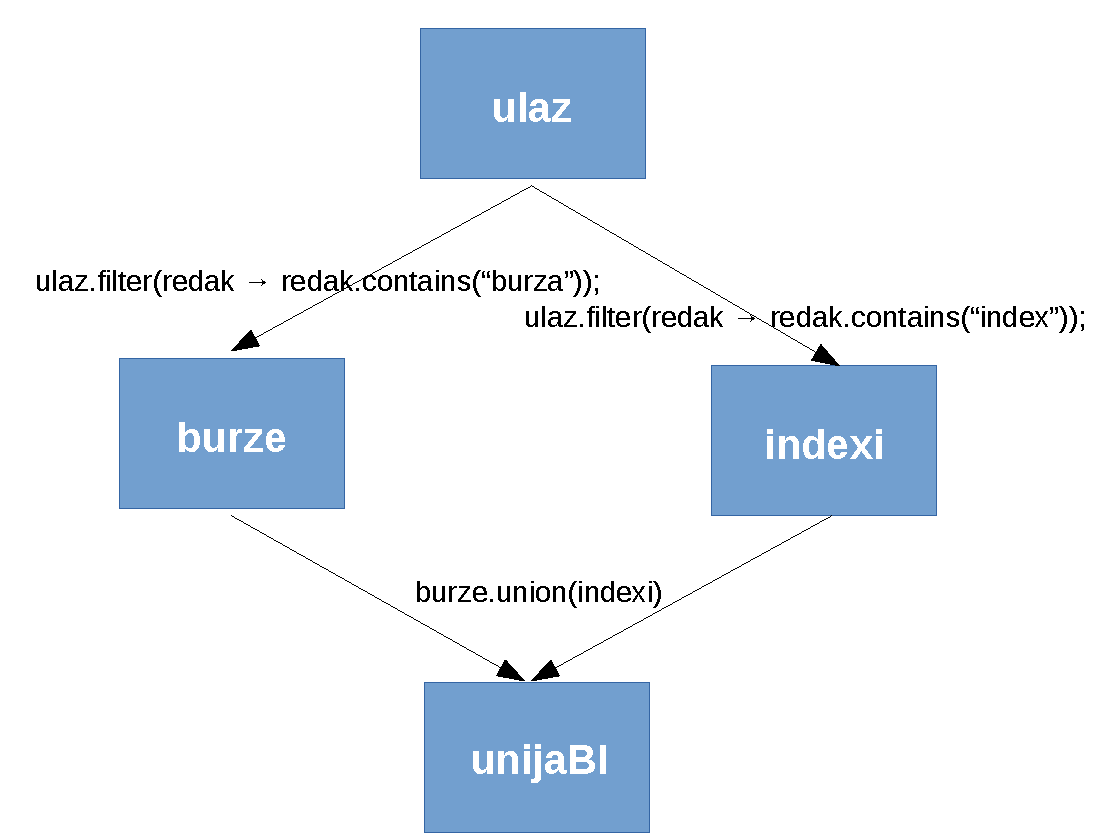
\includegraphics[scale = 0.8]{img/transformacijeCropped.pdf}
\caption{Transformacije nad skupovima podataka.}
\label{fig:burzeUnijaIndexiRDD}
\end{figure}

Tek prilikom poziva akcije \texttt{burzaUnijaIndexi.count()} se zapravo kreira  \texttt{ulaz}, na temelju njega \texttt{burza} i \texttt{indexi} i onda tek na temelju njih se kreira \texttt{unijaBI}. Iz  \texttt{unijaBI} ukupni broj linija dohvati se pozivom \texttt{unijaBI.count()}. 
Nakon što se to izračuna, svi skupovi podataka nestaju iz memorije.  Prilikom poziva akcije \texttt{unijaBI.first()} \textbf{ponovno} se kreiraju prethodno navedeni skupovi podataka i sve ide iz početka.

Na prvi pogled ovo izgleda kao loša implementacija, ali budući da se ovdje radi o velikoj količini podataka i ne možemo ih nikako sve pohraniti u memoriju, ovo je zapravo logična implementacija. 
Ukoliko ne želimo svaki puta iz početka računati i kreirati \texttt{unijaBI}, trebamo ga pohraniti pozivom metode \texttt{persist()} i predavanjem odgovarajućeg parametra. Tablica \ref{tbl:razinePerzistencije} sadrži usporedbu različitih parametara koji se mogu predati metodi \texttt{persist()}.

\begin{table}[htb]
\scriptsize
\caption{Usporedba mogućih parametara za metodu \texttt{persist()}.}
\label{tbl:razinePerzistencije}
\centering
\begin{tabular}{lllll} 
\hline
Razina & Prostorno zauzeće & Procesorsko vrijeme & U memoriji & Na disku\\
\hline
\texttt{MEMORY\_ONLY} & Visoko & Nisko & Da & Ne  \\
\texttt{MEMORY\_ONLY\_SER} & Nisko & Visoko & Da & Ne  \\
\texttt{MEMORY\_AND\_DISK} & Visoko & Srednje & Dio & Dio \\
\texttt{MEMORY\_AND\_DISK\_SER} & Nisko & Visoko & Dio & Dio \\
\texttt{DISK\_ONLY} & Nisko & Visoko & Ne & Da \\
\hline
\end{tabular}
\end{table}

Iz tablice \ref{tbl:razinePerzistencije} očito je da postoje dvije osi usporedbe: spremanje na disk - spremanje u memoriju i spremanje u serijaliziranom obliku - spremanje u neserijaliziranom obliku. Postoji i parametar \texttt{MEMORY\_AND\_DISK} koji prvo podatke sprema u memoriju dok se memorija ne napuni, a kada se napuni, ostatak podataka se sprema na disk. Ono što razlikuje parametre koji sadrže postfiks \texttt{SER} i one koji ga ne sadrže je to što parametri s postfiksom \texttt{SER} spremaju podatke u serijaliziranom obliku, a drugi ne.


\chapter{Napredno programiranje}
U ovom poglavlju opisane su neke napredne tehnike za rad s tehnologijom \emph{Apache Spark}. Objašnjen je algoritam \emph{PageRank}, a dana je i implementacija istog u primjeru \ref{lst:pagerank}.
\section{Primjer: Algoritam PageRank}
Zanimljivo je pitanje kako je \emph{Google} toliko dobar u rezultatima koje korisnik dobije na svoj upit, točnije, kako ispravno sortira po relevantnosti stranice od važnije prema manje važnoj? Odgovor na to daje algoritam \emph{PageRank} koji je dobio ime po jednom od osnivača \emph{Googlea}, Larry Pageu. Ovo potpoglavlje analizira upravo algoritam \emph{PageRank}. U nastavku je iznesena pojednostavljena verzija algoritma, a više informacija o samom algoritmu nalazi se na \url{https://en.wikipedia.org/wiki/PageRank}. 

\subsection{Upoznavanje s algoritmom}
Algoritam računa koliko je koja stranica važna po tome koliko drugih stranica upućuje na nju. Ideja je jednostavna: što više stranica ima poveznicu na neku stranicu \texttt{N}, to je stranica \texttt{N} važnija i time bolje rangirana. U obzir se uzima i koja stranica pokazuje na stranicu \texttt{N} (je li to stranica na koju sve ostale stranice pokazuju ili je to neka stranica na koju nitko ne pokazuje) kao i na koliko ostalih stranica ta stranica sadrži poveznice (nije isto ako je na cijeloj stranici samo jedna poveznica i ako na cijeloj stranici ima 1000 poveznica). Stranice na koje neka stranica \texttt{M} sadrži poveznice nazivamo \emph{susjedima}.

Pojednostavljena izvedba algoritma je sljedeća:
\begin{enumerate}[label*=\arabic*.]
\item Početni rang svake stranice postavi se na $1.0$.
\item Ponavljaj \texttt{P} puta:
\begin{enumerate}[label*=\arabic*.]
\item Svaka stranica \texttt{\emph{n}} svim svojim susjedima šalje doprinos \texttt{rang(\emph{n})/brojSusjeda(\emph{n})}.
\item Postavi ukupni rang stranice prema formuli: $0.15 + 0.85*\emph{ukupan primljeni doprinos}$.
\end{enumerate}
\end{enumerate}

Kako bi se dobio što brže dobio što precizniji rezultat, važno je parametar \texttt{P} postaviti na \emph{ispravnu} vrijednost. U praksi je dovoljno \texttt{P} postaviti na 10. 

Pretpostavimo raspored stranica kao na slici \ref{fig:pageRankSusjedi}.

\begin{figure}[htb]
\centering
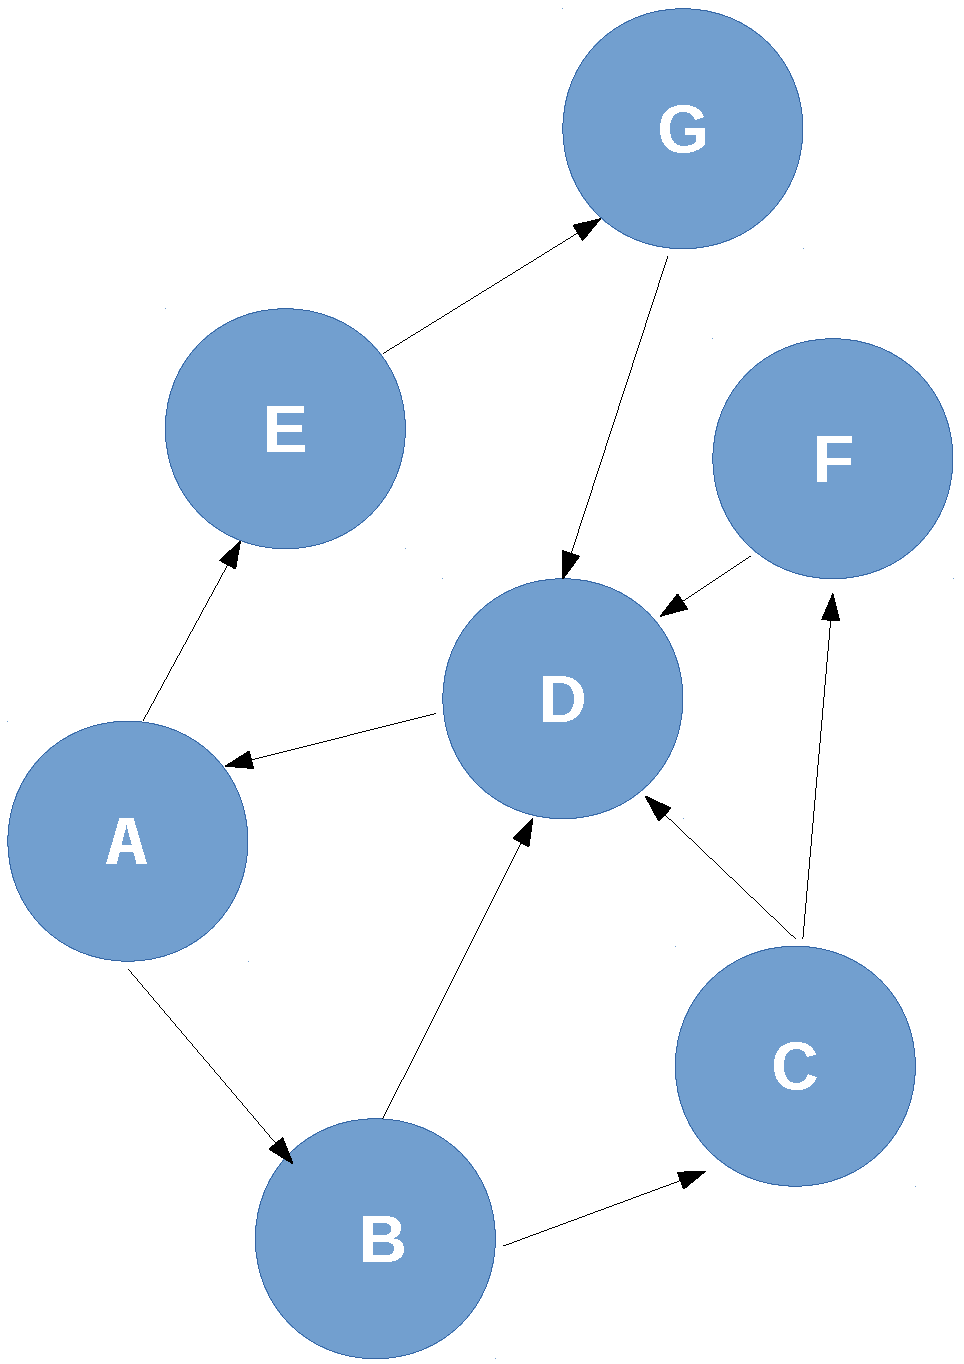
\includegraphics[scale = 0.5]{img/algoritamPageRankRucnoCropped.pdf}
\caption{Raspored susjeda u algoritmu}
\label{fig:pageRankSusjedi}
\end{figure}

U nastavku je raspisan algoritam \emph{PageRank} nad stranicama koje imaju susjede definirane kao na slici \ref{fig:pageRankSusjedi}. Ako stranica \texttt{N} sadrži poveznicu na stranicu \texttt{M} to je na toj istoj slici definirano tako da strelica počinje iz kruga s oznakom \texttt{N}, a vrh joj pokazuje na krug s oznakom \texttt{M}.

Intuitivno se čini da bi stranica \texttt{D} trebala biti najviše rangirana budući da najviše stranica upućuje na nju. Idemo to provjeriti. Za početak, odredimo susjede od svake stranice i postavimo rang svake stranice na $1.0$ kao što je prikazano u tablici \ref{tbl:pageRankKorak1}.
\pagebreak
\begin{table}[htb]
\caption{Inicijalizacija rangova i određivanje susjeda}
\label{tbl:pageRankKorak1}
\centering
\begin{tabular}{lll} 
\hline
Stranica & Rang & Susjedi \\
\hline
A & $1.0$ & B, E\\
B & $1.0$ & C\\
C & $1.0$ & D, F\\
D & $1.0$ & A\\
E & $1.0$ & G\\
F & $1.0$ & D\\
G & $1.0$ & D\\
\hline
\end{tabular}
\end{table}

Sada se ponavljaju koraci 2.1 i 2.2 \texttt{P} puta. Ovdje je ponovljeno 2 puta i to bi trebalo biti dovoljno za razumjevanje algoritma.
Iz koraka 2.1 računa se doprinos koja šalje svaka od stranica. Doprinos stranice \texttt{A} koji šalje drugima iznosi $1.0 / 2 = 0.5$. Doprinos stranice \texttt{B} koji šalje drugima je $1.0 / 2 = 0.5$. Doprinos stranice \texttt{C} jednak je kao i doprinos stranica \texttt{A} i \texttt{B} jer imaju jednak rang i broj susjeda. Doprinos stranica \texttt{D}, \texttt{E}, \texttt{F} i \texttt{G} iznosi $1.0 / 1 = 1.0$. Rezultati za svaku od stranica prikazani su u tablici \ref{tbl:pageRankKorak21p1}.

\begin{table}[htb]
\caption{Izračun doprinosa koji šalje svaka od stranica.}
\label{tbl:pageRankKorak21p1}
\centering
\begin{tabular}{llll} 
\hline
Stranica & Rang & Susjedi & Doprinos drugima\\
\hline
A & $1.0$ & B, E & 0.5\\
B & $1.0$ & C, D & 0.5\\
C & $1.0$ & D, F & 0.5\\
D & $1.0$ & A & 1.0\\
E & $1.0$ & G & 1.0\\
F & $1.0$ & D & 1.0\\
G & $1.0$ & D & 1.0\\
\hline
\end{tabular}
\end{table}

Sada, za svaku od stranica se računa ukupna suma koju je ta stranica dobila od svojih susjeda po formuli dana u koraku 2.2.
Budući da je stranica \texttt{A} susjed samo od stranice \texttt{D}, ukupni primljeni doprinos koji je primila stranica \texttt{A} je upravo doprinos koji stranica \texttt{D} može dati drugima, a to je $1.0$. Stranica \texttt{B} je susjed jedino stranici \texttt{A} i doprinos koji prima je upravo doprinos koji stranica \texttt{A} može u ovom trenutku dati drugima, a to je $0.5$. Stranica \texttt{C} je susjed jedino stranici \texttt{B} i zbog toga je njen ukupni primljeni doprinos $0.5$. Stranica \texttt{D} je susjed stranicama \texttt{B}, \texttt{C}, \texttt{F} i \texttt{G} pa je njen ukupni primljeni doprinos $0.5 + 0.5 + 1.0 + 1.0 = 3.0$. Ukupan primljeni doprinos za svaku od stranica nalazi se u tablici \ref{tbl:pageRankKorak22ap1}.
\pagebreak
\begin{table}[htb]
\caption{Ukupni primljeni doprinos svake od stranica.}
\label{tbl:pageRankKorak22ap1}
\centering
\begin{tabular}{lllll} 
\hline
Stranica & Rang & Susjedi & Doprinos drugima & Ukupni primljeni doprinos\\
\hline
A & $1.0$ & B, E & 0.5 & 1.0\\
B & $1.0$ & C, D & 0.5 & 0.5\\
C & $1.0$ & D, F & 0.5 & 0.5\\
D & $1.0$ & A & 1.0 & 3.0\\
E & $1.0$ & G & 1.0 & 0.5\\
F & $1.0$ & D & 1.0 & 0.5\\
G & $1.0$ & D & 1.0 & 1.0\\
\hline
\end{tabular}
\end{table}

Nakon što je izračunat ukupni primljeni doprinos, vrijeme je za ponovni izračun ranga svake od stanica po formuli koja se nalazi u koraku 2.2. Novi rang stranice \texttt{A} iznosi $0.15 + 0.85 * 1.0 = 1.0$. Novi rang stanice \texttt{B} iznosi $0.15 + 0.85 * 0.5 = 0.575$. Novi rang stranice \texttt{C} iznosi isto $0.575$ jer stranica \texttt{C} i stranica \texttt{B} imaju jednaki ukupni primljeni doprinos. Novi rang stranice \texttt{D} je $0.15 + 0.85 * 3.0 = 2.7$. Nakon što se izračuna i postavi novi rang za svaku od stranica, nastupi situacija kao u tablici \ref{tbl:pageRankStanje1}

\begin{table}[htb]
\caption{Rang svake od stranica nakon prve iteracije.}
\label{tbl:pageRankStanje1}
\centering
\begin{tabular}{lll} 
\hline
Stranica & Rang & Susjedi \\
\hline
A & $1.0$ & B, E\\
B & $0.575$ & C, D\\
C & $0.575$ & D, F\\
D & $2.7$ & A\\
E & $0.575$ & G\\
F & $0.575$ & D\\
G & $1.0$ & D\\
\hline
\end{tabular}
\end{table}

Vidimo da je već u prvoj iteraciji algoritma stranica \texttt{D} iskočila sa svojim rangom od okoline. Ovo smo bili i pretpostavili budući da je stranica \texttt{D} susjed najvećem broju stranica, odnosno najveći broj stranica sadrži poveznicu na stranicu \texttt{D}. 

Idemo napraviti još jednu iteraciju i vidjeti što će se dogoditi s rangovima. 

Iz tablice \ref{tbl:pageRankStanje1} dohvaćamo rang i broj susjeda svake od stranica te računamo doprinos koji svaka od stranica može dati svojim susjedima prema već spomenutoj formuli u gornjem algoritmu u koraku 2.1. Doprinos koji stranica \texttt{A} šalje drugima iznosi $1.0 / 2 = 0.5$. Doprinos koji stranica \texttt{B} šalje je $0.575 / 2 = 0.2875$. Doprinos stranice \texttt{C} je jednak doprinosu stranice \texttt{B} budući da imaju jednak rang i broj susjeda. Doprinos stranice \texttt{D} iznosi $2.7 / 1 = 2.7$. Doprinos stranica \texttt{E} i \texttt{F} iznosi $0.575$, a doprinos stranice \texttt{G} je $1.0$. Rezultati izračuna koliko koja stranica doprinosi drugima prikazani su u tablici \ref{tbl:pageRankKorak21p2}.

\begin{table}[htb]
\caption{Izračun doprinosa koji šalje svaka od stranica u drugoj iteraciji.}
\label{tbl:pageRankKorak21p2}
\centering
\begin{tabular}{llll} 
\hline
Stranica & Rang & Susjedi & Doprinos drugima\\
\hline
A & $1.0$ & B, E & 0.5\\
B & $0.575$ & C, D & 0.2875\\
C & $0.575$ & D, F & 0.2875\\
D & $2.7$ & A & 2.7\\
E & $0.575$ & G & 0.575\\
F & $0.575$ & D & 0.575\\
G & $1.0$ & D & 1.0\\
\hline
\end{tabular}
\end{table}

Sada se ponovno računa ukupni primljeni doprinos svake od stranica. Tako za stranicu \texttt{A} se dobije da ukupni primljeni doprinos iznosi $2.7$ jer je ona jedino susjed stranici D. Ukupni primljeni doprinos stranice \texttt{B} je $0.5$ jer je upravo to iznos koliko stranica \texttt{A} doprinosi drugima, a stranica \texttt{B} je jedino susjed od stranice \texttt{A}. Stranica \texttt{C} ima ukupni primljeni doprinos $0.2875$ jer je upravo to iznos doprinosa stranice \texttt{B}, a stranica \texttt{C} je susjed jedino stranici \texttt{B}. Stranica \texttt{D} prima zbroj doprinosa svih stranica kojima je susjed odnosno zbroj doprinosa stranica \texttt{B}, \texttt{C}, \texttt{F} i \texttt{G}. Iz toga proizlazi da je ukupni primljeni doprinos stranice \texttt{D} $0.2875 + 0.2875 + 0.575 + 1.0 = 2.15$. Ukupni primljeni doprinos za svaku od stranica nalazi se u tablici \ref{tbl:pageRankKorak22ap2} 

\begin{table}[htb]
\caption{Ukupni primljeni doprinos svake od stranica u drugoj tablici.}
\label{tbl:pageRankKorak22ap2}
\centering
\begin{tabular}{lllll} 
\hline
Stranica & Rang & Susjedi & Doprinos drugima & Ukupni primljeni doprinos\\
\hline
A & $1.0$ & B, E & 0.5 & 2.7\\
B & $0.575$ & C, D & 0.2875 & 0.5\\
C & $0.575$ & D, F & 0.2875 & 0.2875\\
D & $2.7$ & A & 2.7 & 2.15\\
E & $0.575$ & G & 0.575 & 0.5\\
F & $0.575$ & D & 0.575 & 0.2875\\
G & $1.0$ & D & 1.0 & 0.575\\
\hline
\end{tabular}
\end{table}

Nakon što je i u drugoj iteraciji izračunat ukupni primljeni doprinos, vrijeme je za ponovni izračun ranga svake od stanica po formuli koja se nalazi u koraku 2.2. Novi rang stranice \texttt{A} iznosi $0.15 + 0.85 * 2.7 = 2.445$. Novi rang stanice \texttt{B} iznosi $0.15 + 0.85 * 0.5 = 0.575$. Novi rang stranice \texttt{C} iznosi $0.15 + 0.85 * 0.2875 = 0.394375 $. Novi rang stranice \texttt{D} je $0.15 + 0.85 * 2.15 = 1.9775$.
Rang stranice \texttt{E} je $0.15 + 0.85 * 0.5 = 0.575$, a rang stranice \texttt{F} iznosi $0.15 + 0.85 * 0.2875 = 0.394375$. Konačno, rang stranice \texttt{G} je $0.15 + 0.85 * 0.575 = 0.63875$. Nakon što se postavi novi rang za svaku od stranica, nastupi situacija kao u tablici \ref{tbl:pageRankStanje2}

\begin{table}[htb]
\caption{Rang svake od stranica nakon prve iteracije.}
\label{tbl:pageRankStanje2}
\centering
\begin{tabular}{lll} 
\hline
Stranica & Rang & Susjedi \\
\hline
A & $2.445$ & B, E\\
B & $0.575$ & C, D\\
C & $0.394375$ & D, F\\
D & $1.9775$ & A\\
E & $0.575$ & G\\
F & $0.394375$ & D\\
G & $0.63875$ & D\\
\hline
\end{tabular}
\end{table}

Iz tablice \ref{tbl:pageRankStanje2} vidljivo je da je stranica \texttt{A} preuzela vodstvo. To se isto može intuitivno prihvatiti budući da skoro sve stranice pokazuju na stranicu \texttt{D}, a upravo \texttt{D} je jedina stranica koja pokazuje na \texttt{A}.

Nakon što se izvrti 10 iteracija, stvari se stabiliziraju. Graf koji opisuje kako se rangovi mijenjaju kroz 10 iteracija prikazan je slikom \ref{fig:grafRangIteracija}.

\begin{figure}[htb]
\centering
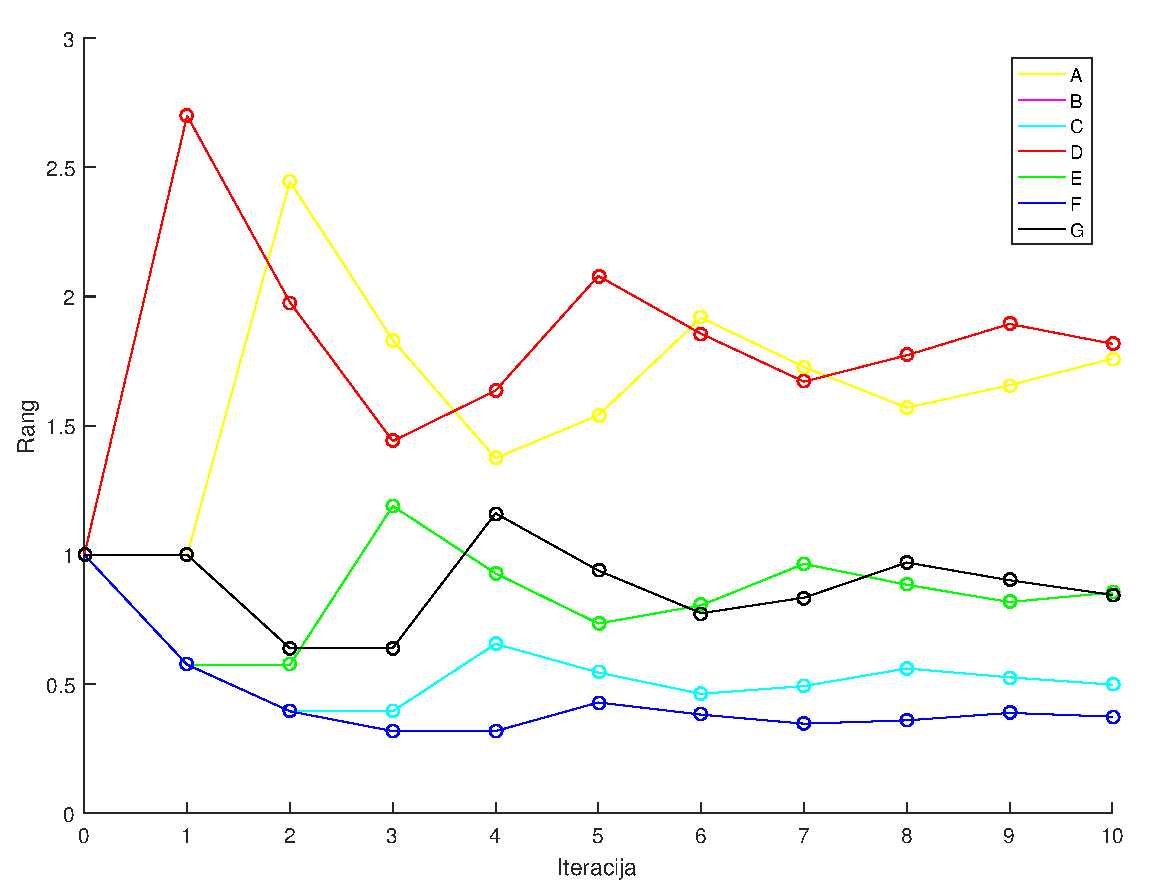
\includegraphics[scale = 0.5]{img/grafPageRankStraniceCropped.pdf}
\caption{Vrijednosti ranga ovisno o iteraciji}
\label{fig:grafRangIteracija}
\end{figure}

\subsection{Implementacija i analiza}
Kada je poznato kako "ručno" radi algoritam, ne bi trebao biti problem napisati programsku implementaciju koja se nalazi u primjeru \ref{lst:pagerank}. U ovom dijelu je osim samog koda napisana i detaljna analiza tog koda kako bi se dobilo što više informacija o tome kako tehnologija \emph{Apache Spark} radi. 

\vspace{5mm}
\begin{lstlisting}[numbers=left, label={lst:pagerank}]
package hr.fer.zemris.naprednoProgramiranje;

import java.util.ArrayList;
import java.util.List;

import org.apache.spark.SparkConf;
import org.apache.spark.api.java.JavaPairRDD;
import org.apache.spark.api.java.JavaRDD;
import org.apache.spark.api.java.JavaSparkContext;

import com.google.common.collect.Iterables;

import scala.Tuple2;

/**
 * Program računa rang pojedine stranice. 
 * Očekuje se da svaki redak ulazne datoteke sadrži 
 * samo 2 stranice u formatu "StranicaA StranicaB", a taj
 * zapis predstavlja da je StranicaB susjed od StranicaA.
 * 
 * @author mmatak
 *
 */
public class AlgoritamPageRank {
	private static final String ULAZNA_DATOTEKA = "pageRankInput.txt";
	private static final int BROJ_ITERACIJA = 10;

	public static void main(String[] args) {
		// Inicijalizacija SparkContext-a.
		SparkConf conf = new SparkConf().setMaster("local")
				.setAppName("Algoritam PageRank");
		JavaSparkContext sc = new JavaSparkContext(conf);

		// Učitavanje podataka.
		JavaRDD<String> ulaz = sc.textFile(ULAZNA_DATOTEKA);

		// Pročitaj sve ulazne URL-e i inicijaliziraj njihove susjede.
		JavaPairRDD<String, Iterable<String>> linkovi = ulaz.mapToPair(
				redak -> {
					String[] elementi = redak.split("\\s+");
					return new Tuple2<String, String>(elementi[0], elementi[1]);
				}).distinct().groupByKey().cache();
		// Svako ime susjeda zamijeni s 1.0 i vrati novi skup podataka.
		JavaPairRDD<String, Double> rangovi = linkovi.mapValues(value -> 1.0);

		// iteracija 2. i 3. koraka algoritma
		for (int i = 0; i < BROJ_ITERACIJA; i++) {
			// za svaki link izracunaj njegovu doprinos drugim linkovima
			JavaPairRDD<String, Double> doprinosi =
			linkovi.join(rangovi).values().flatMapToPair(
				linkoviRang -> {
				
					int brojSusjeda = Iterables.size(linkoviRang._1);
					List<Tuple2<String, Double>> rezultati = new ArrayList<Tuple2<String, Double>>();
					
						for (String susjed : linkoviRang._1) {
							rezultati.add(new Tuple2<String, Double>(
							susjed, linkoviRang._2 / brojSusjeda));
						}
						
						return rezultati;
						
				}
			);
			rangovi = doprinosi.reduceByKey((v1, v2) -> v1 + v2)
					.mapValues(suma -> 0.15 + suma * 0.85);
		}
		// spremi u memoriju
		List<Tuple2<String, Double>> rangoviFinal = rangovi.collect();
		// ispis
		for (Tuple2<String, Double> entry : rangoviFinal) {
			System.out.printf("Stranica %s ima rang %.2f\n", entry._1, entry._2);
		}
		sc.close();
	}
}
\end{lstlisting}
\captionof{lstlisting}{Algoritam \emph{PageRank}.}
\vspace{5mm}
TODO: Analiza gore implementiranog algoritma. 
\section{RDD-i kao uređeni parovi}
\section{Čitanje i spremanje podataka}
\section{Globalne varijable}
\chapter{Zaključak} 
Zaključak.


\begin{thebibliography}{9}
\bibitem{officialDocumentation}
  Službena dokumentacija projekta \emph{Apache Spark} \url{http://spark.apache.org/docs/latest/} , posjećeno 1.5.2016
\bibitem{learningSpark}
  Holden Karau, Andy Konwinski, Patrick Wendell i Matei Zaharia
  \emph{Learning Spark, lighting-fast}, O'Reilly 2015.
\bibitem{marcupic}
  Marko Čupić,
  \emph{Programiranje u Javi},
  verzija 0.3.26
\bibitem{workingSets}
  Matei Zaharia, Mosharaf Chowdhury, Michael J. Franklin, Scott Shenker, Ion Stoica,
  \emph{Spark: Cluster Computing with Working Sets}, University of California, Berkeley
\end{thebibliography}

\newpage
% Dodatak nije obavezan
\begin{appendices}
\chapter{Instalacija}
\label{ch:instalacijaSpark}
Ovdje će biti prikazana instalacija na operacijskom sustavu \emph{Ubuntu 15.10}. Ovo nije veliko ograničenje jer se iz ovih uputa može zaključiti i kako instalacija ide za neki drugi operacijski sustav.

Za početak je potrebno imati instaliranu Javu, a je li Java instalirana na računalu se može provjeriti tako što se u naredbenom retku unese sljedeća naredba:\\
\texttt{java -version}. Kao rezultat bi trebali dobiti trenutno instaliranu verziju Jave. Ukoliko Java nije instalirana, potrebno ju je najprije instalirati. Više informacija o instalaciji se može pronaći u \cite{marcupic}.

Jednom kada imamo instaliranu Javu, sve što treba napraviti je otići na službene stranice: \url{https://spark.apache.org/downloads.html}, odabrati najnoviju verziju (Za vrijeme pisanja ovog rada to je verzija \emph{1.6.1 (Mar 09 2016}), izabrati odgovarajući paket te pokrenuti dohvaćanje odgovarajuće \emph{.tgz} arhive. Najjednostavnije je odabrati neki \emph{pre-built} paket, primjerice \emph{Pre-built for Hadoop 2.6 and later}. Daljnji koraci instalacije su napisani pod pretpostavkom da je dohvaćena ta verzija paketa. Moguće je instalirati i \emph{Source code} varijantu paketa, ali taj postupak instalacije ovdje nije opisan. 

Nakon što je dohvaćena odgovarajuća arhivu, potrebno ju je raspakirati.\\ Raspakiranje arhive moguće je napraviti preko naredbe:
\begin{lstlisting}[language=bash]
$ tar -xvf spark-1.6.1-bin-hadoop2.6.tgz
\end{lstlisting}
Nakon toga, dobra je praksa premjestiti instalaciju u neki prikladniji direktorij. Tako nešto može se napraviti na sljedeći način:
\begin{lstlisting}[language=bash]
$ mv Downloads/spark-1.6.1-bin-hadoop2.6 faks/spark/
\end{lstlisting}
Ovim korakom je instalacija završena. 

Kako bi bili sigurni da je instalacija uspješna, potrebno je pozicionirati se u \emph{bin} direktorij te u terminalu upisati \texttt{./spark-shell}. Ispis bi trebao biti sličan ovome:\\
\begin{lstlisting}[language=bash]
mmatak@martins-beast:~/faks/spark/bin$ ./spark-shell
Welcome to
      ____              __
     / __/__  ___ _____/ /__
    _\ \/ _ \/ _ `/ __/  '_/
   /___/ .__/\_,_/_/ /_/\_\   version 1.6.1
      /_/

Using Scala version 2.10.5 (OpenJDK 64-Bit Server VM, Java 1.8.0_91)
Type in expressions to have them evaluated.
Type :help for more information.
scala>
\end{lstlisting}


Ukoliko se prikaže greška vezana uz \emph{sqlContext}, to nije razlog za brigu. U ovom trenutku to nije važno. Radi ljepšeg formata ovog rada, u gornjem ispisu izbrisana su upozorenja \engl{warnings}.
\chapter{Postavljanje datoteke pom.xml}
\label{ch:datotekapomXML}
Datoteka koja je potrebna kako bi Maven ispravno dohvatio artifakt \texttt{spark-core} bi trebala izgledati slično kao što je dano u nastavku. Za ispravno funkcioniranje, trebala bi se zvati \texttt{pom.xml}.
\begin{lstlisting}[language=XML]
<project xmlns="http://maven.apache.org/POM/4.0.0" xmlns:xsi="http://www.w3.org/2001/XMLSchema-instance" xsi:schemaLocation="http://maven.apache.org/POM/4.0.0 http://maven.apache.org/xsd/maven-4.0.0.xsd">
  <modelVersion>4.0.0</modelVersion>
  <groupId>hr.fer.zemris</groupId>
  <artifactId>Prvi-programi</artifactId>
  <version>0.0.1-SNAPSHOT</version>
  <name>Prvi programi</name>
  <description>Prvi programi u Spark-u</description>
  <dependencies>
  	<dependency>
  		<groupId>org.apache.spark</groupId>
  		<artifactId>spark-core_2.10</artifactId>
  		<version>1.6.1</version>
  	</dependency>
  </dependencies>
</project>
\end{lstlisting}
\end{appendices}

\begin{sazetak}
Sažetak na hrvatskom jeziku.

\kljucnerijeci{Ključne riječi, odvojene zarezima.}
\end{sazetak}

% TODO: Navedite naslov na engleskom jeziku.
\engtitle{Title}
\begin{abstract}
Abstract.

\keywords{Keywords.}
\end{abstract}

\end{document}
